\FloatBarrier
\section{Optimization mechanism and systems cost}
\label{sec:mechanism_cost}

\paragraph{From loss gains to update geometry and runtime.}
We next examine how structure-aware output factors change individual parameter updates and multi-checkpoint cotangent trajectories, and measure the remaining step-time overhead across GPU counts.

\subsection{Output factors rotate updates with little norm change}
\label{sec:mechanism}

\paragraph{Counterfactual step-norm invariance.}
To isolate the immediate action of the output operator, we hold checkpoint momentum and input factors fixed and recompute counterfactual updates under identity (\mname{MuonT}), all-diagonal (\mname{Muon2-Diag}), and expansion-diagonal (\mname{Muon2-ExpDiag}) output factors on saved 130M (32 layers, step 2,500) and 520M ($\eta^*=0.016$, 16 layers, step 5,120) checkpoints (\Cref{tab:mechanism_rotation}, \Cref{fig:mech_pareto}(a)). Across projections, \mname{Muon2-ExpDiag} update Frobenius norms stay at $0.985\times$ their input-only counterparts at 130M and $1.006\times$ at 520M, ruling out global step-size inflation.

\paragraph{Stiefel frame rotation from inner whitening.}
An exact row-polar identity shows why inner whitening rotates the update even after singular values are equalized. For a full-row-rank pre-polar matrix $Z_0=UR=S_0P_0$ with $m\le n$, $S_0\succ0$, and $P_0P_0^{\Tr}=I_m$, left-multiplying by $L\succ0$ gives
\begin{equation}
 \operatorname{Polar}(LZ_0)=\Omega P_0,\qquad
 \Omega=(LS_0^2L)^{-1/2}LS_0\in SO(m).
 \label{eq:som_rotation}
\end{equation}
Whenever $L$ and $S_0$ do not commute, $\Omega$ rotates the orthogonal row frame tangentially along the Stiefel manifold, while post-multiplying by symmetric $\hat L$ scales output directions orthogonally in first-order Frobenius inner product ($\tr(HK^{\Tr})=0$ for symmetric $H$ and skew-symmetric $K$; derivations and empirical inner/outer angles for finite $\Nten$ and tall matrices appear in \Cref{app:appendix_mech,tab:rotation_detail}).

\begin{table}[!htb]\centering\small
\setlength{\tabcolsep}{4.5pt}
\caption{\textbf{Counterfactual update rotation, top-mode de-hijacking, and width scaling across 130M (32-layer means) and 520M (16-layer means).} Holding checkpoint momentum and input factors fixed, $\theta_{\rm WT}$ and $\theta_{\rm OD}$ measure update angles relative to input-only updates ($\|D_{\rm WT}\|_F/\|D_{\rm MT}\|_F = 0.985$ at 130M and $1.006$ at 520M). Hijack reports top-16 overlap between pre-polar momentum singular vectors and $B_t$ eigenvectors before and after inner whitening; DA is 520M median diagonal anisotropy share (residual $\mathrm{IPR}=3.02$); $\Phi$ ratios are directional quadratic proxies relative to MuonT, not measured loss gains. At 520M, \texttt{gate,up} track 1D diagonals online ($\text{WT}=\text{OD}$).}\label{tab:mechanism_rotation}
\begin{tabularx}{\textwidth}{@{}>{\raggedright\arraybackslash}Xrrrrrrrrr@{}}
\toprule
& \multicolumn{4}{c}{130M ($\dm=512$, step 2,500)} & \multicolumn{5}{c}{520M ($\dm=1{,}024$, step 5,120)} \\
\cmidrule(lr){2-5}\cmidrule(lr){6-10}
Output & Hijack & $\theta_{\rm WT}$ & $\theta_{\rm OD}$ & $\Phi_{\rm WT}/\Phi_{\rm MT}$ & DA & $\theta_{\rm WT}$ & $\theta_{\rm OD}$ & $\Phi_{\rm WT}/\Phi_{\rm MT}$ & $\Phi_{\rm OD}/\Phi_{\rm MT}$ \\
\midrule
q & $67.8\to2.8\%$ & $22.7^\circ$ & $20.8^\circ$ & 1.155 & 9.8\% & $24.0^\circ$ & $22.7^\circ$ & 1.625 & 1.182 \\
k & $64.2\to3.7\%$ & $22.6^\circ$ & $22.8^\circ$ & 1.233 & 16.8\% & $24.8^\circ$ & $24.5^\circ$ & 1.737 & 1.247 \\
v & $19.6\to1.1\%$ & $24.2^\circ$ & $17.2^\circ$ & 1.264 & 0.7\% & $25.1^\circ$ & $16.5^\circ$ & 3.341 & 1.137 \\
\addlinespace[2.5pt]
\rowcolor{rowtint}[0pt][0pt]\textbf{o} (res.) & $30.4\to3.5\%$ & $15.5^\circ$ & $3.9^\circ$ & 1.002 & 0.5\% & $\mathbf{15.4^\circ}$ & $6.4^\circ$ & \textbf{1.334} & 1.028 \\
\rowcolor{rowtint}[0pt][0pt]\textbf{down} (res.) & $64.5\to2.8\%$ & $15.7^\circ$ & $5.1^\circ$ & 1.098 & 0.4\% & $\mathbf{14.6^\circ}$ & $6.0^\circ$ & \textbf{1.263} & 1.009 \\
\addlinespace[2.5pt]
gate & $22.7\to3.1\%$ & $15.9^\circ$ & $15.9^\circ$ & 1.292 & --- & $18.8^\circ$ & $18.8^\circ$ & --- & --- \\
up & $33.7\to4.7\%$ & $16.4^\circ$ & $16.4^\circ$ & 1.249 & --- & $18.6^\circ$ & $18.6^\circ$ & --- & --- \\
\bottomrule\end{tabularx}
\end{table}


\begin{figure}[t]
 \centering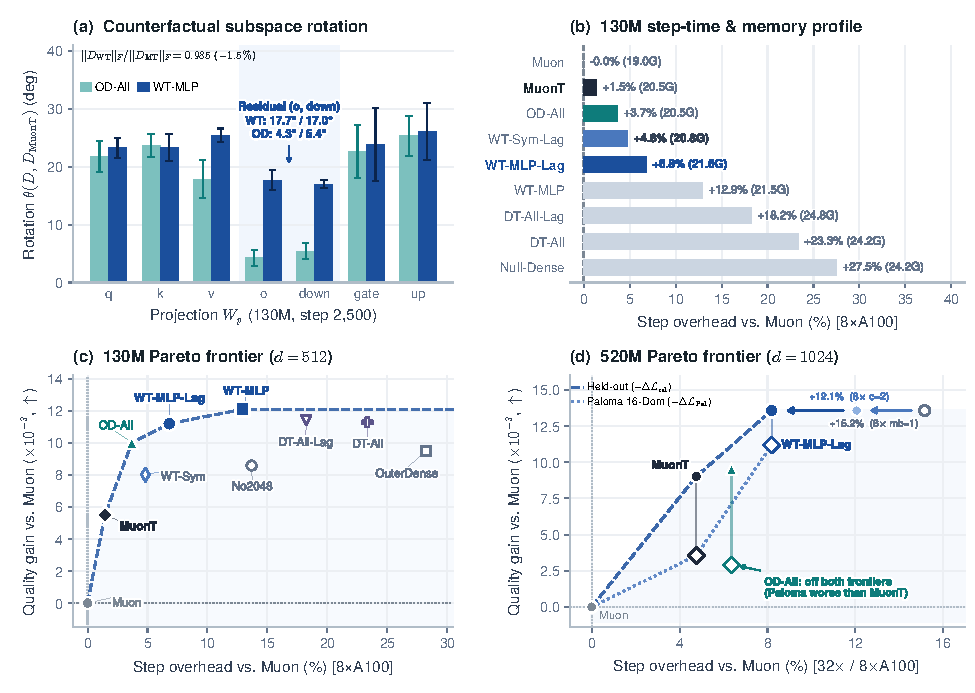
\includegraphics[width=\textwidth]{fig8_mechanism_and_pareto.pdf}
 \caption{\textbf{Dense output factors rotate residual-stream updates while retaining a bounded runtime cost.}
 \textbf{(a)} Counterfactual update rotation relative to input-only updates at 130M, step 2,500 (each arm on its own trained state; bars show 32-layer means and whiskers $\pm1$ SD; common-state probes at both widths are in \Cref{tab:mechanism_rotation}).
 \textbf{(b)} 130M median step-time overhead versus \mname{Muon} and per-GPU peak memory on $8\times\text{A100}$.
 \textbf{(c, d)} Quality gain versus median step-time overhead at 130M ($8\times\text{A100}$) and 520M ($32\times$ and $8\times\text{A100}$). Frontiers combine fixed-token losses with steady-step timing benchmarks rather than wall-clock time to a target loss.}
 \label{fig:mech_pareto}
\end{figure}

\paragraph{Residual update rotation and singular-frame de-hijacking.}
On the 520M checkpoint, \mname{Muon2-ExpDiag} rotates the residual-stream \texttt{o} and \texttt{down} updates by $15.4^\circ$ and $14.6^\circ$, compared with $6.4^\circ$ and $6.0^\circ$ under \mname{Muon2-Diag} (\Cref{tab:mechanism_rotation}). At 130M, inner whitening cuts top-16 overlap between pre-polar momentum singular vectors and dominant $B_t$ eigenvectors from $30\text{--}68\%$ to $2.8\text{--}3.7\%$ ($19.6\to1.1\%$ on \texttt{v}) while raising row alignment across 69--82\% of the trailing 80\% of output modes (\Cref{tab:rotation_detail}). Structure-aware updates also raise the directional quadratic score $\Phi_{B,C}(\hat D)=\langle U,\hat D\rangle^2/\tr(\tilde B\hat D\tilde C\hat D^{\Tr})$ over \mname{MuonT}. Because observed-label cotangent moments are not true Hessians or model Fishers~\citep{kunstner2019limitations} (and \mname{GO-MUON} can score high on $\Phi_{B,C}$ despite poor training loss), these probes describe update geometry rather than proving causal generalization gains.

\paragraph{Eigenvector delocalization across model width.}
Coordinate scaling misses more of these residual rotations as width grows because residual-output eigenvectors are spread across coordinates. Their median normalized inverse participation ratio is $d\sum_i u_i^4\approx 3.01\text{--}3.02$ at both widths, close to the Haar-random benchmark $3d/(d+2)$. Under a reference model with Haar-distributed eigenvectors and fixed non-isotropic eigenvalues, expected diagonal anisotropy decays inversely with width:
\begin{equation}
 \E_{U\sim\mathrm{Haar}}[\mathrm{DiagAniso}(U\Lambda U^{\Tr})]=\frac{2}{d+2},
 \label{eq:haar_scaling}
\end{equation}
matching the observed drop in residual-output diagonal share from $\approx 0.8\%$ at $\dm=512$ to $0.45\%$ at $\dm=1{,}024$.

\subsection{Trajectory-level reduction in output-subspace drift}
\label{sec:output_drift}

\paragraph{Fixed-data subspace-drift protocol.}
Training with \mname{Muon2-ExpDiag} also slows the temporal drift of leading output-cotangent subspaces across saved checkpoints (\Cref{tab:output_drift}, \Cref{fig:output_drift}). To compare all seven output roles on shared data without minibatch-order noise, we evaluate each saved checkpoint passively on two disjoint fixed sets $\mathcal S$ of 4,576 token positions (16 windows of 4,096 tokens each) to form $B_t^{\mathcal S}=|\mathcal S|^{-1}\sum_{s\in\mathcal S}\delta_t(s)\delta_t(s)^{\Tr}$ for each projection. Between consecutive checkpoints, we measure principal-angle subspace drift $D_k(t_1,t_2)=1-\|V_{t_1}^{\Tr}V_{t_2}\|_F^2/k$ at $k=16$ (full protocol, per-role curves, EMA audit, and sensitivity checks in \Cref{app:drift_details,fig:output_drift_roles}).

\begin{table}[tbp]\centering\footnotesize
\setlength{\tabcolsep}{5pt}
\caption{\textbf{Output-subspace drift with Muon as the baseline.} Fixed-data top-16 drift, averaged equally over 32 layers, two probe sets, and 19 intervals of 250 steps at 130M or three intervals of 2,560 steps at 520M. At 520M and in fresh 130M seeds 1--3 (one 2,560--5,120 interval per seed), all three methods share $\eta=0.016$; the densely saved 130M seed-0 trajectories use $0.016$ for Muon and $0.02263$ for MuonT/WT, so that column does not isolate optimizer effects at a common rate. Reductions are $100(1-\overline D_{\rm method}/\overline D_{\rm Muon})$; positive values mean lower drift than Muon. Seed summaries are mean $\pm$ sample SD across three seeds. The all-role row averages drift before taking ratios; absolute drift is not compared across model sizes. WT denotes WT-MLP-Lag.}\label{tab:output_drift}
\begin{tabularx}{\textwidth}{@{}>{\raggedright\arraybackslash}X*{6}{>{\raggedleft\arraybackslash}X}@{}}\toprule
& \multicolumn{3}{c}{130M: absolute drift} & \multicolumn{3}{c}{520M: absolute drift} \\
\cmidrule(lr){2-4}\cmidrule(lr){5-7}
Output & Muon & MuonT & WT & Muon & MuonT & WT \\\midrule
\texttt{q} & 0.363 & 0.368 & 0.304 & 0.352 & 0.348 & 0.277 \\
\texttt{k} & 0.399 & 0.390 & 0.366 & 0.494 & 0.469 & 0.431 \\
\texttt{v} & 0.565 & 0.614 & 0.591 & 0.771 & 0.762 & 0.745 \\
\texttt{o} & 0.335 & 0.360 & 0.284 & 0.529 & 0.461 & 0.410 \\
\texttt{down} & 0.313 & 0.342 & 0.276 & 0.493 & 0.426 & 0.393 \\
\texttt{gate} & 0.682 & 0.677 & 0.522 & 0.863 & 0.837 & 0.665 \\
\texttt{up} & 0.583 & 0.583 & 0.358 & 0.764 & 0.746 & 0.471 \\
\midrule
All roles & 0.463 & 0.476 & 0.386 & 0.609 & 0.579 & 0.485 \\
\bottomrule\end{tabularx}
\par\vspace{6pt}
\begin{tabularx}{\textwidth}{@{}>{\raggedright\arraybackslash}Xrrrrrr@{}}\toprule
& \multicolumn{2}{c}{130M: reduction (\%)} & \multicolumn{2}{c}{520M: reduction (\%)} & \multicolumn{2}{c}{130M seeds 1--3: reduction (\%)} \\
\cmidrule(lr){2-3}\cmidrule(lr){4-5}\cmidrule(lr){6-7}
Output & MuonT & WT & MuonT & WT & MuonT & WT \\\midrule
\texttt{q} & -1.6 & +16.2 & +1.1 & +21.3 & $+2.7\pm1.1$ & $+17.5\pm2.7$ \\
\texttt{k} & +2.3 & +8.4 & +5.1 & +12.7 & $+5.9\pm1.5$ & $+8.9\pm0.8$ \\
\texttt{v} & -8.7 & -4.6 & +1.1 & +3.3 & $+2.0\pm0.6$ & $+3.2\pm0.8$ \\
\texttt{o} & -7.4 & +15.2 & +12.8 & +22.6 & $+2.2\pm6.3$ & $+19.2\pm2.1$ \\
\texttt{down} & -9.0 & +12.1 & +13.6 & +20.4 & $+1.4\pm7.9$ & $+16.4\pm1.9$ \\
\texttt{gate} & +0.7 & +23.6 & +3.0 & +22.9 & $+5.3\pm2.3$ & $+22.6\pm1.1$ \\
\texttt{up} & 0.0 & +38.6 & +2.3 & +38.4 & $+2.7\pm3.2$ & $+39.5\pm0.8$ \\
\midrule
All roles & -2.9 & +16.7 & +5.1 & +20.5 & $+3.3\pm2.9$ & $+18.8\pm0.6$ \\
\bottomrule\end{tabularx}
\end{table}


\begin{figure}[tbp]
 \centering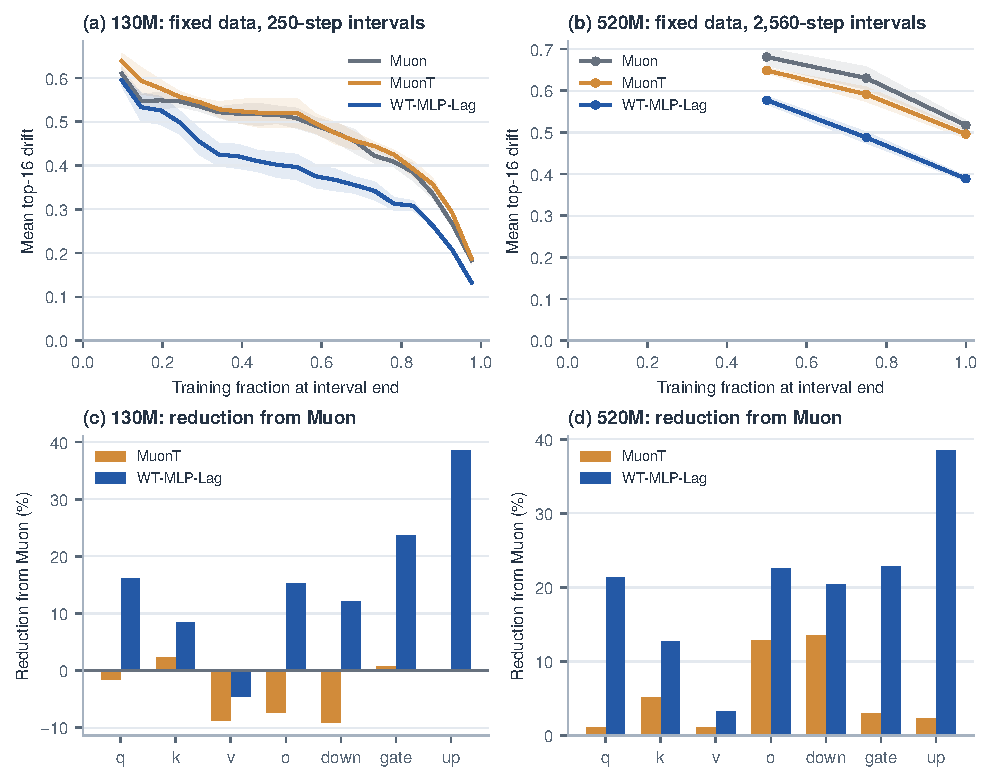
\includegraphics[width=\textwidth]{fig9_output_drift.pdf}
 \caption{\textbf{\mname{Muon2-ExpDiag} reduces leading output-subspace drift across 130M and 520M training trajectories.}
 \textbf{(a, b)} Fixed-data top-16 cotangent-subspace drift across saved \mname{Muon}, \mname{MuonT}, and \mname{Muon2-ExpDiag} checkpoints, averaged over seven output roles, 32 layers, and two disjoint probe sets (shading spans the two probe-set means; 19 intervals of 250 steps at 130M and three 2,560-step intervals at 520M).
 \textbf{(c, d)} Role-wise percentage drift reduction relative to \mname{Muon}. All three 520M runs share $\eta=0.016$, whereas 130M seed-0 runs use $\eta=0.016$ for \mname{Muon} and $\eta=0.02263$ for \mname{MuonT} and \mname{Muon2-ExpDiag}; matched-rate fresh-seed checks appear in \Cref{tab:output_drift}.}
 \label{fig:output_drift}
\end{figure}

\paragraph{Drift reductions across 130M and 520M trajectories.}
Relative to \mname{Muon}, \mname{Muon2-ExpDiag} lowers all-role mean top-16 drift by 16.7\% across 19 equal 250-step intervals at 130M ($0.463\to0.386$, whereas \mname{MuonT} is $2.9\%$ higher at $0.476$), and by 20.5\% across the three 2,560-step intervals covering the final three quarters of matched-rate ($\eta=0.016$) 520M training ($0.609\to0.485$, versus $0.579$ or $+5.1\%$ reduction for \mname{MuonT}). Reductions are largest on \texttt{gate} ($23.6\%,22.9\%$) and \texttt{up} ($38.6\%,38.4\%$); at 520M every role decreases in every interval (including $+3.3\%$ on \texttt{v}), whereas on the mixed-rate 130M seed-0 curve \texttt{v} sits $-4.6\%$ higher than \mname{Muon}. Relative to \mname{MuonT}, \mname{Muon2-ExpDiag} lowers all-role drift by 19.0\% at 130M and 16.2\% at 520M, improving every role in every equal-length interval. Because the densely saved 130M seed-0 runs use $\eta=0.016$ for \mname{Muon} and $\eta=0.02263$ for \mname{MuonT} and \mname{Muon2-ExpDiag}, we also check the three fresh 130M seeds at matched $\eta=0.016$ (steps 2,560--5,120): as at 520M, \mname{Muon2-ExpDiag} reduces drift relative to \mname{Muon} across all seven roles on every seed, averaging $18.8\pm0.6\%$ overall versus $3.3\pm2.9\%$ for \mname{MuonT}.

\paragraph{Training-EMA and rank-sensitivity checks.}
Uninterrupted 130M training-EMA checkpoints relative to a passive \mname{MuonT} control confirm lower average top-16 drift across all five saved dense output roles ($16.3\%,12.0\%,11.4\%,7.8\%,28.0\%$ on \texttt{q,k,v,o,down}), while qualifying \Cref{tab:diagnosis_summary}'s resumed replay window where uninterrupted steps 2,250--2,500 are slightly higher on \texttt{o,down} ($0.138,0.109$ versus $0.134,0.107$) despite lower full-run averages. Fixed-data sign patterns also hold across $k\in\{8,16,32,64\}$ and under a 1\% eigenvalue-gap filter (\Cref{app:drift_details}). These audits measure trajectory subspace stability; they do not establish that lower drift causes lower held-out loss or permits slower root refreshes.

\subsection{Step-time overhead and token-versus-time tradeoff}
\label{sec:pareto}

\paragraph{Median step-time waterfall across GPU scales.}
Expansion-output diagonalization and one-step overlap remove most, though not all, of two-sided runtime cost (\Cref{tab:timing_summary}, \Cref{fig:mech_pareto}(b--d); excluding compilation, evaluation, and checkpoint I/O). On matched 130M checkpoints ($8\times\text{A100}$), input-only \mname{MuonT} adds $+1.5\%$ median step time over \mname{Muon} and synchronous dense outputs (\mname{Muon2-Dense}) add $+23.3\%$; diagonalizing \texttt{gate,up} (\mname{Muon2-ExpDiag (sync)}) cuts total overhead to $+12.9\%$, and one-step lag (\mname{Muon2-ExpDiag}) lowers it to $+6.8\%$ ($+5.3\%$ above \mname{MuonT}). At 520M across $32\times\text{A100}$, matched-checkpoint median overhead over \mname{Muon} is $+4.8\%$ for \mname{MuonT} and $+8.2\%$ for \mname{Muon2-ExpDiag} ($+3.3\%$ above \mname{MuonT}).

\begin{table}[!htb]\centering\small
\setlength{\tabcolsep}{5.8pt}
\caption{\textbf{Step-time co-design waterfall and multi-node scaling (both median and mean estimators).} Overheads ($\Delta$) are relative to same-group Muon using the matching estimator (matching \Cref{fig:overview}(b) and \Cref{fig:mech_pareto}(b--d)); Peak GiB is per-GPU peak allocated memory. Expansion-output diagonalization and one-step lag cut total two-sided median overhead from $+23.3\%$ (Muon2-Dense) to $+6.8\%$ at 130M ($+5.3\%$ above MuonT) and $+8.2\%$ at 520M ($+3.3\%$ above MuonT), while retaining a slower mean tail from periodic basis repairs. Complete 130M and 520M configurations appear in \Cref{tab:bench19,tab:bench520m}.}\label{tab:timing_summary}
\begin{tabularx}{\textwidth}{@{}>{\raggedright\arraybackslash}Xrrrrr@{}}
\toprule
Configuration / Method & Median (s) & Median $\Delta$ & Mean (s) & Mean $\Delta$ & Peak GiB \\
\midrule
\addlinespace[2pt]\multicolumn{6}{@{}l}{\textit{130M co-design progression: 8 GPUs, 0.5M batch, matched checkpoint (steps 37--96)}}\\
Muon (reference) & 1.081 & $+0.0\%$ & 1.079 & $+0.0\%$ & 18.97 \\
MuonT (input only) & 1.097 & $+1.5\%$ & 1.097 & $+1.7\%$ & 20.54 \\
Muon2-Diag (all outputs diagonal) & 1.121 & $+3.7\%$ & 1.120 & $+3.7\%$ & 20.55 \\
Muon2-Dense (all outputs dense, sync) & 1.333 & $+23.3\%$ & 1.459 & $+35.2\%$ & 24.21 \\
Muon2-ExpDiag (sync, $\tau=0$) & 1.221 & $+12.9\%$ & 1.250 & $+15.8\%$ & 21.52 \\
\rowcolor{rowtint}[0pt][0pt]\textbf{Muon2-ExpDiag ($\tau=1$ lag)} & \textbf{1.155} & $\mathbf{+6.8\%}$ & \textbf{1.194} & $\mathbf{+10.7\%}$ & \textbf{21.60} \\
\addlinespace[5pt]\multicolumn{6}{@{}l}{\textit{520M width and cluster scaling: 32 GPUs, 1.0M batch, chunked buffers}}\\
Muon (matched ckpt, ref.) & 1.322 & $+0.0\%$ & 1.324 & $+0.0\%$ & 26.46 \\
MuonT (matched ckpt) & 1.385 & $+4.8\%$ & 1.391 & $+5.1\%$ & 26.93 \\
Muon2-Diag (matched ckpt) & 1.406 & $+6.4\%$ & 1.412 & $+6.6\%$ & 26.94 \\
\rowcolor{rowtint}[0pt][0pt]\textbf{Muon2-ExpDiag (matched ckpt)} & \textbf{1.430} & $\mathbf{+8.2\%}$ & \textbf{1.549} & $\mathbf{+17.0\%}$ & \textbf{27.88} \\
Muon2-ExpDiag (warm vs.\ warm Muon) & 1.458 & $+11.1\%$ & 1.539 & $+16.9\%$ & 27.88 \\
\bottomrule\end{tabularx}
\end{table}


\paragraph{Upper-tail repair cost and wall-clock tradeoff.}
Periodic fallback eigendecompositions leave a heavier upper tail in mean step times: relative to \mname{Muon}, the same matched benchmarks record mean overheads of $+10.7\%$ at 130M and $+17.0\%$ at 520M, or $+8.9\%$ and $+11.4\%$ above \mname{MuonT} ($+11.1\%$ median and $+16.9\%$ mean vs.\ warm \mname{Muon}, or $+5.6\%$ and $+11.1\%$ above warm \mname{MuonT}, when resuming each method's own warmed 520M state on 32 GPUs; complete 8- and 32-GPU windows in \Cref{tab:bench19,tab:bench520m}). At a recorded 130M C4 target of $3.52$ nats, \mname{Muon2-ExpDiag} reaches the target in $5.3\%$ fewer tokens than \mname{MuonT} (step 4,501 vs.\ 4,751; $2.36\text{B}$ vs.\ $2.49\text{B}$ tokens) but $1.8\%$ more elapsed wall-clock time ($5{,}564.6$ vs.\ $5{,}468.4$\,s). Our experiments therefore establish a fixed-token quality improvement while leaving net wall-clock speedups open.
